\documentclass[a4paper,twoside,10pt]{article}
\interfootnotelinepenalty=10000
\usepackage[USenglish]{babel} %francais, polish, spanish, ...
\usepackage[T1]{fontenc}
%\usepackage[ansinew]{inputenc}
\usepackage{color}
\usepackage{mathtools}
%\usepackage{hyperref}
\usepackage{subfig}
\usepackage{multirow, booktabs}
\usepackage{hyperref}


\usepackage{lmodern} %Type1-font for non-english texts and characters
\usepackage{algorithm}
\usepackage[noend]{algpseudocode}
\usepackage{mnsymbol}

%% Packages for Graphics & Figures %%%%%%%%%%%%%%%%%%%%%%%%%%
\usepackage{graphicx} %%For loading graphic files
\usepackage{amsmath}
\usepackage{amsthm} 
\usepackage{thmtools}
\usepackage{amsfonts}
\usepackage[all,cmtip]{xy}
\usepackage{tikz}

\usepackage{TechFront}
%\declaretheorem{Lemma}
%\declaretheorem{prop}

\newcommand{\lre}{\color{red}{\{}}

%\DeclareMathOperator{\sign}{sgn}
%\DeclareMathOperator{\coef}{coef}
%\DeclareMathOperator{\var}{var}
%\DeclareMathOperator{\eqs}{eqs}
%\DeclareMathOperator{\feas}{feas}
%\DeclareMathOperator{\UB}{UB}
%\DeclareMathOperator{\lb}{lb}
%\DeclareMathOperator{\FMcomb}{FM-comb}
%\DeclareMathOperator{\Gcomb}{Gauss-comb}
%\DeclareMathOperator{\proj}{proj}
%\DeclareMathOperator{\Pos}{Pos}
%\DeclareMathOperator{\Neg}{Neg}
%\DeclareMathOperator{\rhs}{rhs}
\newcommand{\sign}{\mathit{sgn}}
\newcommand{\coef}{\mathit{co}}
\newcommand{\var}{\mathit{var}}
\newcommand{\VAR}{\mathit{VAR}}
\newcommand{\eqs}{\mathit{eqs}}
\newcommand{\feas}{\mathit{feas}}
\newcommand{\UB}{\mathit{UB}}
\newcommand{\UBc}{\mathit{UBineq}}
\newcommand{\lb}{\mathit{lb}}
\newcommand{\lbc}{\mathit{lbineq}}
\newcommand{\FMcomb}{\mathit{FM}}
\newcommand{\Gcomb}{\mathit{GA}}
\newcommand{\proj}{\mathit{proj}}
\newcommand{\Pos}{\mathit{Pos}}
\newcommand{\Neg}{\mathit{Neg}}
\newcommand{\rhs}{\mathit{rhs}}
\newcommand{\bounds}{\mathit{bounds}}
\newcommand{\ie}{\mathcal{IE}}
\newcommand{\xx}{\mathcal{X}}
\newcommand{\vea}{\mathbf{co}}
\newcommand{\ttt}{\texttt{t}}
\newcommand{\trt}[1]{\texttt{#1}}
\newcommand{\mi}{\mathit}

\newcommand{\false}{\texttt{false}}
\newcommand{\true}{\texttt{true}}
\newcommand{\nul}{\texttt{null}}
\newcommand{\ve}{\mathbf}
%\newcommand\lhs[1]{\text{lhs}(#1)}
%\newcommand\rhs[1]{\text{rhs}(#1)}
%\newcommand\coef[1]{\text{coef}(#1)}
%\newcommand\LB[1]{\text{LB}_{#1}}
%\newcommand\UB[1]{\text{UB}_{#1}}
\newcommand{\lig}[4]{\ve{#1}\cdot\ve{#2}#3#4}
\newcommand\red[1]{\textcolor{red}{#1}}
\newcommand\blue[1]{\textcolor{blue}{#1}}
\newcommand{\set}[2]{\{\;{#1}\;|\;{#2}\;\}}
\newcommand{\odef}{\overset{\text{def.}}=}
\newcommand{\mc}{\mathcal}
\algdef{SE}[DOWHILE]{Do}{doWhile}{\algorithmicdo}[1]{\algorithmicwhile\ #1}%
\newcommand{\argmin}{\operatornamewithlimits{argmin}}
\newcommand{\StateInd}{\State\hspace{\algorithmicindent}}
\newcommand{\pr}{\mathit{PR}}
\newcommand{\prs}{\mathit{PRS}}
\newcommand{\ens}{\Leftrightarrow}

%\algdef{SE}[DOPAR]{DoPar}{doParWhile}{\algorithmicdo\textbf{ in parallel for\ }}[1]{\algorithmicwhile\ #1}%
\algdef{SE}[DOPAR]{DoPar}{doParUntil}{\algorithmicdo\textbf{ in parallel for\ }}[1]{\algorithmicuntil\ #1}%

\algdef{SE}[SUBALG]{Indent}{EndIndent}{}{\algorithmicend\ }%
\algtext*{Indent}
\algtext*{EndIndent}

\newtheorem{prop}{Proposition}
\newtheorem{lemma}{Lemma}
\newtheorem{cor}{Corollary}

\newcounter{para}
%\newcommand\mypara[1]{\par\refstepcounter{para}\textbf{\thep‌​ara\space#1\space}}
\newcommand\mypara[1]{\newline\par\refstepcounter{para}\textbf{\thepara}\space \textbf{#1} \space}
%\newcommand\mypara{\par\refstepcounter{para}\thepara\space}
%\usepackage[thmmarks,...]{ntheorem}
\newcommand{\Sec}{F}
\newcommand{\Ca}{\mi{Cap}}
\newcommand{\Vol}{\mi{V}}
\newcommand{\Weight}{\mi{W}}
\newcommand{\weight}{\mi{w}}
\newcommand{\BonjeanStations}{\mi{BS}}
\newcommand{\bonjean}{bf}
\newcommand{\Bonj}{B}
\newcommand{\shear}{\mi{sf}}
\newcommand{\Prop}{P}

\theoremstyle{definition}
%\newtheorem{example}{Example}[section]
\newtheorem*{theorem}{Theorem}

\theoremstyle{definition}
\newtheorem{examplex}{Example}[section]
\newenvironment{example}
  {\pushQED{\qed}\renewcommand{\qedsymbol}{$\triangle$}\examplex}
  {\popQED\endexamplex}
	
%\newtheoremstyle{named}{}{}{\itshape}{}{\bfseries}{.}{.5em}{\thmnote{#3}}
%\theoremstyle{named}
%\newtheorem*{namedtheorem}{Theorem}

\usepackage{longtable}
\newcounter{counterName}
\allowdisplaybreaks
\begin{document}

\Ttitle{A Decomposed Fourier-Motzkin Elimination Framework to Derive Capacity Models of Container Vessels}
\Tauthors{Mai L. Ajspur, Rune M. Jensen, and Kent H. Andersen}
  
\maketitle

\begin{abstract}
Accurate capacity models expressing the trade-off between different container types that can be stowed
on vessels are required in core liner shipping functions such as uptake-, capacity-, and network management.
Today, simple capacity models are used for these tasks, which causes overestimations. 
Though previous work on stowage planning optimization in principle provide fine-grained Vessel Stowage Models (VSMs), they are too complex to be used in the mentioned functions. 
As an alternative, this article contributes a novel framework based on Fourier-Motzkin
elimination that automatically derives Vessel Capacity Models (VCMs) from VSMs by projecting unneeded
variables. Our results show that the projected VCMs are reduced by an order of magnitude both in number of
inequalities and number of non-zero entries and can be solved up to 20-35 times faster than their corresponding VSMs with only a negligible loss in accuracy. 
Our framework is applicable to LP models in general, but are particularly effective on block-angular structured problems such as VSMs. We show similar results for a multi-commodity flow problem.
\end{abstract}


\section{Introduction}
Container shipping is a central element in the clockwork of global trade \cite{EC13}. A container liner shipping company operates a set of container vessels which sail on closed loop services with fixed schedules. These services connect major trade regions like Asia and Europe, and the liner shipping business is focused on utilizing the cargo capacity in their service network. Unused capacity constitute a loss that can be fatal in a market with a profit margin of just a few percent.  
To maximize utilization of capacity, it is central for a liner shipping company to be able to estimate the residual capacity of a container vessel. This is challenging in practice. For an air plane, an empty seat usually means that the plane can fit an extra passenger. For a container vessel, on the other hand, an empty slot may be impossible to utilize for a wide range of reasons. For instance, if the slot can be loaded with a container within the weight and volume limits of its stack, the container may exhaust the lashing gear or cause the vessel to be unstable or exceed its stress limits. Moreover, it may block containers below it to be discharged in earlier ports, ruin the utilization of quay cranes, be in conflict with stowage rules or segregation rules for dangerous cargo, or obstruct the view of the captain. 

The various stowage rules and seaworthiness requirements interact such that the free capacity of each container type and weight class is a complex function of the composition of cargo on board and the design of the vessel. Often it is only the stowage planning team that can determine the residual capacity of a vessel accurately, and even they may sometimes have to manually construct a stowage condition of the vessel to be able to do it. While stowage planners may be able to estimate free vessel capacity, the knowledge is primarily needed in higher order functions such as: {\em uptake management} that control the sale of cargo bookings to fill the vessels with profitable cargo; {\em capacity management} that route cargo through the service network; {\em network management} that makes changes to the service network; and {\em fleet management} that charters and buys vessels for the service network and reposition vessels between closing and opening services. Decision makers in these functions seldom have stowage insight or time to consult the stowage team. They usually boil down the free capacity of a vessel to its nominal volume, weight, and reefer (refrigerated containers) capacity minus total volume, weight and reefer number of containers already on board. This simple three dimensional capacity model is inherently optimistic, since it ignores stowage complications. It has been shown that it can lead to revenue over-estimates of more than 15\% \cite{AlbertosThesis}. This can cause sub-optimal decisions that significantly harm business.

In this article, we present a method to calculate a Vessel Capacity Model (VCM) automatically from a linear Vessel Stowage Model (VSM) based on previous research on stowage optimization \cite{pacino11,AlbertosThesis}. 
The basic idea is to derive the VCM by abstracting away the slot position of containers in the VSM so that the model only expresses the relationship between the residual capacity of each possible container type.
Inspired by previous work in constraint programming (e.g., \cite{lassez90}) and software verification (e.g., \cite{benoy05}), we do this by projecting container position variables out of the mentioned stowage models using a framework based on Fourier-Motzkin Elimination (FME). Similar to other recent FME frameworks (e.g., \cite{simon05,lukatskii08,shapot12}), our framework includes additional features such as using equalities for substitutions (Gauss-elimination), removing syntactically redundant constraints, a complete removal of redundant constraint after each variable elimination, and a method for coarsening the boundary of the projection. Our main computational contribution is a novel decomposition method that takes advantage of block-angular structured models to significantly speed-up the projection of variables in these models. Additionally, the complete redundancy is parallellized, and the framework includes preprocessing of the constraint system including removal of less strict inequalities.

Our experimental evaluation of computing VCMs with this method shows that FME generates a large number of redundant constraints in each projection iteration that can be removed. In theory, the number of non-redundant constraints can grow exponentially with the number of projected variables \cite{monniaux10}. However, the number of constraints and non-zeros in the resulting capacity models typically are reduced by an order of magnitude compared to their corresponding stowage models. Moreover, the decomposition method reduces the size of the intermediary models produced by FME, causing less time to be needed for removing redundant constraints, which again speeds up the projection process significantly. In addition, for the models that include hydrostatic constraints, the resulting VCMs can be solved 20-35 times faster than their VSMs with only a negligible loss in accuracy. Although it can take several hours to derive a capacity model due to the clean-up of redundant constraints, this only has to be done one time for a vessel class. In this way, the approach is suitable for computing capacity models that can be applied in higher order functions of liner shipping companies such as uptake-, capacity-, fleet-, and network management. Moreover, since they are linear and much faster to solve than their corresponding stowage models, they also can be integrated in decision support systems used to optimise these functions.

Multi-commodity flow problems also have a block-angular structure, so our framework applies to these problems as well. We assume that the goal is to model how the amount of each commodity at the sinks depends on the amount of the commodities at the sources. For this purpose, the amount of each commodity that flows on edges is irrelevant and eliminated from the system. 
For this projection, we found a speed-up and a reduction in size of the resulting models similar to the ones seen for VCMs.

This article is organized as follows. Section~\ref{sec:background} provides a background on container vessels and stowage rules. Section~\ref{sec:stowmodel} presents the VSM that will later be projected to the wanted VCM. Section~\ref{sec:solutionMethod} outlines the methods used in our FME framework. Section~\ref{sec:results} presents experimental results. Finally, Section~\ref{sec:preWork} gives an overview of related work and Section~\ref{sec:concl} concludes.



\section{Background} \label{sec:background}

The cargo space of a container vessel is divided into parts called \textit{bays} that each consists of a grid of \emph{cells}. Each cell is divided into two \emph{slots} and can accordingly hold one standard $40'$ container or two $20'$ containers. Some cells have power plugs allowing for \emph{reefer} containers to be refrigerated as required. Each bay is divided into three or four parts called \textit{locations}, at which level the vessel's capacities are given. See Figure~\ref{fig:vessel}.

\begin{figure}[htbp]
	\centering
		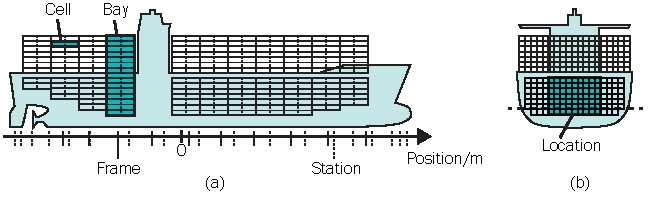
\includegraphics{figures/vessel3.pdf}
	\caption{Vessel structure and reference points seen (a) on a longitudinal intersection and (b) on a transversal intersection.}
	\label{fig:vessel}
\end{figure}

To define common reference points for cargo-holding structures and hydrostatic constraints, we further define larger \emph{sections} of the vessel and their endpoints. Each of these sections either span a number of succeeding bays, or a part of the ship containing no bays at all.
See Figure~\ref{fig:sectionEndPoints}. Note that this is \emph{not} part of the data describing the vessel itself, but an input we define.

\begin{figure}[htbp]
	\centering
		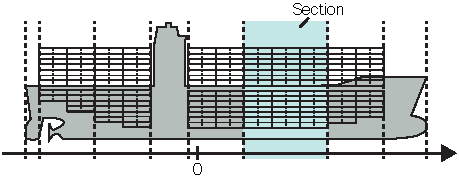
\includegraphics{figures/sectionEndPoints.pdf}
	\caption{Sections on a vessel. Their endpoints are used as common reference points for cargo-holding structures and hydrostatic constraints in the VSMs.}
	\label{fig:sectionEndPoints}
\end{figure}

An empty vessel without cargo, ballast or equipment is referred to as \emph{lightship}.  The lightship is given in the data by a set of ``blocks'' placed along the vessel. Each block has a given weight that is assumed to be uniformly distributed along the block.
The cargo itself is described by a container \emph{type}, which is defined by a length ($20'$ or $40'$)\footnote{$45'$ long containers are also common, but for the sake of simplicity, we only consider $20'$ and $40'$ containers in this article.}, whether it is a reefer-container or not, and a weight class (in a discrete set of average weights). 
Besides cargo bays, vessels also have \emph{ballast tanks} in fixed positions along the vessel that can be filled with water to improve the stability of the vessel.

Though containers physically are placed in specific slots, the vessel data specifies capacities for each location. These capacities are given in \emph{TEU} (Twenty-foot Equivalent Units), i.e. a standard $20'$ container takes up one TEU, while a $40'$ container takes up two TEU. For each location, the vessel data includes upper bounds for: the total number of TEUs, $20'$ containers, $40'$ containers, reefer slots, reefer cells, plus separate total weight limit for $20'$ and $40'$ containers, respectively. The latter exist, since only $20'$ containers rest on the middle support posts of the stack it is in, while the end posts hold weight of both $20'$ and $40'$ containers. This may lead to different weight capacities of $20'$ and $40'$ containers. Limits for each ballast tank are likewise given in the input data, as well as a limit for the total displacement, i.e. the weight of the vessel, including ballast water, cargo and the ship itself. 

On a vessel, stress forces arise as a result of gravitation acting downwards and buoyancy acting upwards. This results in shear forces and bending moments along the longitudinal axis of the vessel, and limits on these are given for a set of reference points along the vessel called \emph{frames} (see Figure~\ref{fig:vessel}(a)). The buoyancy force comes from the vessel's displacement of water and hence depends on the varying (and irregular) shape of the hull and the displacement of the vessel. The area submerged in water is given at another set of reference points called \emph{stations} for a discrete set of displacement values (see Figure~\ref{fig:vessel}(a)).
The position of these reference points do not line up with bay endpoints, and this is remedied in the Vessel Stowage Model presented in the next section to allow for a less complex modelling. Further requirements to ensure the stability of the vessel are imposed in real life and considered e.g. in \cite{AlbertosThesis}, but are not included here.

\section{Vessel Stowage Model (VSM)} \label{sec:stowmodel}
This section presents the Vessel Stowage Model (VSM) that will be projected to obtain the wanted Vessel Capacity Model (VCM). The model is adapted from work by Delgado (\cite{AlbertosThesis}). It relies on vessel data from a real vessel profile used by an industrial loading computer. The VSM includes various stowage constraints and further describes the hydrostatic constraints reasonably accurate while abstracting away much of the unnecessary complexity relating to the physical layout of the vessel that is present in the data. More specifically, the buoyancy data used in hydrostatic calculations are given at a set of points along the vessel (stations), while hydrostatic constraints are given in relation to another set of points (frames), and neither of these coincide with the position of the structures holding the cargo or the ballast tanks (see Figure~\ref{fig:vessel}(a)). The measure points are aligned in the VSM (see Figure~\ref{fig:sectionEndPoints}), and calculations for the hydrostatic constraints are simplified. 

The sets, variables and parameters used in VSM are listed below. Buoyancy data and hydrostatic limits are translated to the sections' end points, and the derived parameters are included.

\vspace{3mm}
\begin{centering}
\begin{tabular}{p{2.6cm}p{4.8cm}|p{2.4cm}p{4.8cm}}
\multicolumn{2}{l}{\textbf{Sets}}\\
\hline\noalign{\smallskip}
$L$  																	& Locations. 												& $T$	 																	& Types of containers.\\ 
$S$	 																	& Sections (ordered set).						& $T^{\{\trt{20},\trt{R}\}}\subseteq T$ & $20'$ long/reefer types, respectively. \\
$S^{\{\trt{f}, \trt{a}\}}\subseteq S$ & Sections fore/aft, respectively. 	& $\mi{BT}$ 														& Ballast tanks. \\
$L_s\subseteq L$ 											& Locations in section $s\in S$. 		& $F$	 																	& Frames.\\
$B$ 																	& Blocks with constant weight. 			& $\mi{ST}$ 														& Stations.\\
																			&																		& $D$																		& Displacement values.\\
\end{tabular}
\end{centering}
\begin{longtable}
{p{3.7cm}p{11.5cm}}
\multicolumn{2}{l}{\textbf{Decision variables}}\\
\hline\noalign{\smallskip}
$x_{l,\tau}\in \mathbb{R}^+_0$		& {Number of containers of type $\tau\in T$ to be stowed in location $l\in L$}.\\
$t_s\in \mathbb{R}^+_0$						& {The weight of ballast tanks within section $s\in S$.}\\
\\
\multicolumn{2}{l}{\textbf{Auxilliary variables}}\\
\hline\noalign{\smallskip}
$x_\tau\in \mathbb{R}^+_0$ 				& {The total number of containers of type $\tau\in T$.}\\
$w_s\in \mathbb{R}^+_0$						& {The weight of section $s\in S$, everything included.}\\
$w\in \mathbb{R}^+_0$							& {The total displacement (weight).}\\
$b_{s,d} \in\mathbb{R}^+_0$ 			& {The buoyancy force for section $s \in S$ with a total displacement of $d\in \mathbb{R}$.}\\
$\mi{sf}_s\in \mathbb{R}$ 				& {The shear force at the aft endpoint of section $s\in S$.}\\
$\mi{bm}_s\in \mathbb{R}$ 				& {The bending moment at the aft endpoint of section $s\in S$.}\\
\\
\multicolumn{2}{l}{\textbf{Parameters}}\\
\hline\noalign{\smallskip}
$C_l^{\{\trt{20}, \trt{40}, \trt{TEU}\}}\in \mathbb{N}$ 		& {The capacity in TEU for location $l\in L$ w.r.t. $20'$ containers/$40'$ container/TEUs in total, respectively.} \\
$C_l^{\{\trt{RS}, \trt{RC}\}}\in \mathbb{N}$								& {The number of reefer slots/reefer cells in location $l\in L$, respectively.}\\
$C_l^{\{\trt{W20}, \trt{W40}\}}\in \mathbb{N}$							& {The weight capacity of  $20'$/$40'$ containers in location $l\in L$, respectively.}\\
$W_\tau, W_b\in \mathbb{R}^+_0$															& {The weight of container type $\tau\in T$, and of block $b\in B$, respectively.} \\
$A_{\sigma, d}\in \mathbb{R}^+_0$ 													&	{The area submerged in water at station $\sigma\in ST$ for a displacement $d\in D$.}\\
$P^{\{\trt{f},\trt{a}\}}_{l}$, $P^{\{\trt{f},\trt{a}\}}_{b}$, $P^{\{\trt{f},\trt{a}\}}_{t}\in \mathbb{R}$, 
																														&	{The longitudinal position of the fore/aft endpoint of location $l\in L$, block $b \in B$, and tank $t \in BT$, 
																														  respectively.}\\
$P_{f}$, $P_{\sigma}\in\mathbb{R}$ 
																														&	{The longitudinal position of frame $f \in F$, and of station $\sigma\in \mi{ST}$, respectively.}\\
$\mi{Max}^\trt{W}$, $\mi{Max}^\trt{WT}_b\in \mathbb{R}^+$		&	{Upper bound for the total displacement and for ballast tank $b\in BT$, respectively.}\\
$\mi{SF}^{\{+,-\}}_f$, $\mi{BM}^{\{+,-\}}_f\in\mathbb{R}$ 	&	{Upper/lower bounds for the shear force and bending moment at each frame $f\in F$, respectively.}\\
\\
\multicolumn{2}{l}{\textbf{Derived parameters}}\\
\hline\noalign{\smallskip}
$P^{\{\trt{f},\trt{a}\}}_s \in \mathbb{R}$ 									& {The fore/aft position of section $s \in S$.}\\  
$\mi{SF}^{\{+,-\}}_s$, $\mi{BM}^{\{+,-\}}_s\in\mathbb{R}$		& {Upper/lower bounds for the shear force and bending moment, respectively, at the aft endpoint of section $s\in S$.}\\
$\mi{Max}^\trt{WT}_s\in \mathbb{R}$													& {Upper bound for the weight of ballast tanks in section $s\in S$.}\\
$A''_{p, d}\in \mathbb{R}^+_0$															&	{Approximation of the area submerged in water at a longitudinal position $p$ along the vessel for a displacement $d\in \mathbb{R}$.}\\
$\mi{PR}_{b,s}\in[0;1]$																			& {The percentage of the tank $b\in\mi{BT}$ that lies within section $s\in S$.}
\end{longtable}
 A container type $\tau \in T$ defines the container's length (20' or 40'), weight class (6, 21, or 27 tons), and whether it is a reefer or not. The set of stations, $ST$, includes $\sigma^\trt{a}$ and $\sigma^\trt{f}$, which are two (artificial) stations at the aft most and fore most positions of the ship, respectively. Similarly, $F$ contains the frames $f^\trt{a}$ and $f^\trt{f}$. The submerged areas for these stations and bounds for these frames are trivial. It is assumed that if $L_s\neq \emptyset$ then $L_s$ contains all locations that are positioned within some interval on the longitudinal axis. 

The decision variables of the VSM are $x_{l,\tau}$ for all $l\in L$ and $\tau \in T$, denoting the number of containers of type $\tau$ stowed in location $l$, and $t_s$ for all $s\in S$, denoting the amount of ballast water in ballast tanks in section $s$. Even though $x_{l,\tau}$ is a number of containers and hence a natural number, we model it as a real number to ensure that the resulting model is a polyhedron. The auxiliary variables, $x_\tau$ for all $\tau\in T$ are the decision variables of the VCM. All other variables will be eliminated when we transform a VSM into its corresponding VCM. Hence, as required, a capacity model describes the free capacity trade-off between the different container types irrespective of where the containers are stowed on the vessel. The polyhedron representation of the VSM is defined by the following linear equations:
\begin{align}
	\label{typeDef}
	&x_\tau = \sum_{l\in L} x_{l,\tau} 
			&& \forall{\tau \in T}.\\
	%
		\label{20Cap}
	&\smashoperator[r]{\sum_{\tau \in T^\trt{20}}} x_{l,\tau} \leq C_l^\trt{20}
			&& \forall l \in L.\\
	%
	\label{40Cap}    	
	&\smashoperator[r]{\sum_{\tau \in T\setminus T^\trt{20}}} 2\cdot x_{l,\tau} \leq C_l^\trt{40} 
			&& \forall l \in L.\\
	%
	\label{teuCap}
	&\smashoperator[r]{\sum_{\tau \in T^\trt{20}}} x_{l,\tau} + 2\cdot\smashoperator[lr]{\sum_{\tau \in T\setminus T^\trt{20}}} x_{l,\tau} \leq C_l^\trt{TEU} 
			&& \forall l \in L.\\
	%
	\label{weight20Cap}
	&\smashoperator[r]{\sum_{\tau \in T^\trt{20}}} W_\tau\cdot x_{l,\tau} \leq C_l^\trt{W20} 
			&& \forall l \in L.\\
	%
	\label{weight40Cap}
	&\smashoperator[r]{\sum_{\tau \in T\setminus T^\trt{20}}} W_\tau\cdot x_{l,\tau} \leq C_l^\trt{W40} 
			&& \forall l \in L. \\
	%
	\label{combinedWeightCap}
	&0.5 \smashoperator[lr]{\sum_{\tau \in T^\trt{20}}} W_\tau\cdot x_{l,\tau} + \smashoperator[lr]{\sum_{\tau \in T\setminus \in T^\trt{20}}} W_\tau\cdot x_{l,\tau} \leq C_l^\trt{W40} 
			&& \forall l \in L.\\
	%
	\label{reeferSlotCap}
	&\smashoperator[r]{\sum_{\tau \in T^\trt{R}}} x_{l,\tau} \leq C_l^\trt{RS} 
			&& \forall l \in L. \\
	%
	\label{reeferCellCap}
	&\smashoperator[lr]{\sum_{\tau \in T^\trt{R}\cap T^\trt{20}}} 0.5\cdot x_{l,\tau} + \smashoperator[lr]{\sum_{\tau \in T^\trt{R}\setminus T^\trt{20}}} x_{l,\tau} \leq C_l^\trt{RC} 
			&& \forall l \in L.\\
	%
	\label{totalWeightDef}
	&w_s = \sum_{\tau \in T} \sum_{l\in L_s} W_\tau\, x_{l,\tau} + xt_s + \sum_{b\in B} \mi{PR}_{b,s}\cdot W_b 
			&& \forall s \in S.\\
	%
	\label{totalDisp}
	&w  = \sum_{s\in S} w_s. 
			&&\\
	%
	\label{btLim}
	&0 \leq t_s \leq \sum_{b \in BT} \mi{PR}_{b,s}\cdot \mi{Max}^\trt{WT}_b 
			&& \forall s\in S.\\
	%
	\label{xPos}
	&0 \leq x_{l,\tau} 
			&& \forall l\in L, \tau\in T.\\
	%
	\label{wTotalLim}
	&w \leq \mi{Max}^\trt{W}. 
			&&\\
	%
	\label{defBancy}
	&b_{s,d} = \smashoperator[lr]{\sum_{p \in Q\setminus \{P^\trt{f}_s\}}} 0.5\cdot(A''_{p,d}+A''_{\mi{next}_p,d})\cdot (\mi{next}_p-p), 
			&& \forall s\in S, d\in \mathbb{R}.\\%\text{where } \mi{next}_p = \min\set{p' \in P}{p' > p}.\\
	%
	\label{sfF}
	&\mi{sf}_s = \smashoperator[r]{\sum_{s' \in S. P^\texttt{f}_{s'} \geq P^\texttt{f}_s}} (w_{s'} - b_{s',w}) 
			&& \forall s \in S^\texttt{f}.\\
	\label{sfA}
	&\mi{sf}_s = \smashoperator[r]{\sum_{s' \in S. P^\texttt{a}_{s'} < P^\texttt{a}_s}} (w_{s'} - b_{s',w}) 
			&& \forall s \in S^\texttt{a}.\\
	%
	\label{sfLim}
	&\mi{SF}^-_s \leq \mi{sf}_s \leq \mi{SF}^+_s
			&& \forall s \in S.\\
	%
	\label{bmF}
	&\mi{bm}_s = 	\smashoperator[r]{\sum_{s' \in S. P^\texttt{f}_{s'} \geq P^\texttt{f}_s}} (w_{s'} + b_{s',w})\cdot |P^\trt{a}_s - \frac{P^\trt{f}_{s'}-P^\trt{a}_{s'}}{2}|
			&& \forall s \in S^\texttt{f}.\\
	%
	\label{bmA}
	&\mi{bm}_s = \smashoperator[r]{\sum_{s' \in S. P^\texttt{a}_{s'} < P^\texttt{a}_s}} (w_{s'} + b_{s',w})\cdot |P^\trt{a}_s - \frac{P^\trt{f}_{s'}-P^\trt{a}_{s'}}{2}|
			&& \forall s \in S^\texttt{a}.\\
	%
	\label{bmLim}
	&\mi{BM}^-_s \leq \mi{bm}_s \leq \mi{BM}^+_s 
			&& \forall s \in S. 
\end{align}

Equation \eqref{typeDef} defines the decision variables of the VCM. Equations \eqref{20Cap}-\eqref{weight40Cap} ensure that for each location of the vessel, the stowed containers are within the allowed capacities w.r.t. the number of $20'$ containers, $40'$ containers, TEUs, and the weight of the $20'$ and $40'$ containers, respectively.
Likewise, equation \eqref{combinedWeightCap} ensures that the weight of a location is within limits, taken the different distribution of the weight of $40'$ containers, respectively $20'$ containers, within a slot into consideration. Equations \eqref{reeferSlotCap} and \eqref{reeferCellCap} ensure that there is enough reefer plugs for reefer containers. 

For defining the weight of a section, we need its fore and aft position. For \emph{cargo-containing sections}, i.e. sections $s$ for which $L_s\neq \emptyset$, we can find immediate fore- and aft points of the locations in $s$: $P^\trt{if}_s = \max\set{P^\trt{f}_l}{l\in L_s}$, and $P^\trt{ia}_s = \min\set{P^\trt{a}_l}{l\in L_s}$ (see Figure~\ref{fig:sections}). There is a small gap between two consecutive bays, and this space is divided evenly between two consecutive, cargo-containing sections. Sections that are not cargo-containing get their endpoints from the immediate end points of their neighbor sections if these are cargo-containing, and otherwise the non-cargo-containing parts of the vessel is divided evenly among the corresponding non-cargo-containing sections. See Figure~\ref{fig:sections}.
\begin{figure}[htbp]
	\centering
		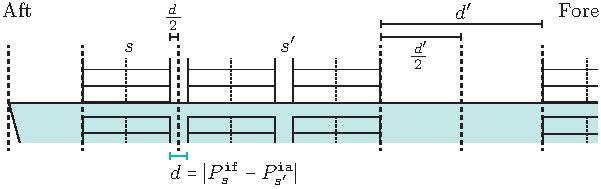
\includegraphics{figures/sections.pdf}
	\caption{The doted lines indicates the endpoints of the sections.}
	\label{fig:sections}
\end{figure}
Using the end points of the sections, equation \eqref{totalWeightDef} defines the total weight of section $s\in S$, including cargo, ballast tanks and the vessel itself. Equation \eqref{totalDisp} defines the total displacement (weight) of the vessel.  Here, $\mi{PR}_{b,s}$ defines the percentage of tank $b$ that lies within section $s\in S$, that is 
\[
\mi{PR}_{b,s} = \frac{\max(\min(P^\texttt{f}_b, P^\texttt{f}_s)-\max(P^\texttt{a}_b, P^\texttt{a}_s),0)}{P^\texttt{a}_s-P^\texttt{f}_s}.
\]

Capacities for individual tanks are pooled into capacities for tanks within a section, such that the amount of ballast water in any section $s$ is limited by the amount of water in the portion of each tank that lies within that section combined, and further it is required to be non-negative \eqref{btLim}. Likewise, the number of containers of each type placed in each section is non-negative \eqref{xPos}. Finally, the total displacement (weight) is required to be within limits \eqref{wTotalLim}.

For a station $\sigma\in\mi{ST}$, the submerged area of the cross-section for a given displacement $d\in D$ is given by $A_{\sigma,d}$. From these values we make an approximation of the submerged area at $\sigma$ for any positive displacement $d\in \mathbb{R}_o^+$. This is done by linearizing the values between the maximal displacement value given in the table, $d_\mi{max}=\text{max}\{d\in D\}$, and a displacement value $d_\mi{min}$ at the point, where the hull does not curve too much anymore. For the cross-section given in Figure~\ref{fig:vessel}(b) this would correspond to the displacement giving rise to the marked waterline. We note that since our VSM will mainly be used for some sort of maximization of loaded cargo it is fair to assume that the displacement will be above the found $d_\mi{min}$. Thus, the approximation of the submerged area is  
\[
A'_{\sigma,d} = \frac{A_{\sigma,d_{max}} - A_{\sigma,d_{min}}}{d_{max} - d_{min}} \cdot (\mi{w} - d_{max}) + A_{\sigma,d_{max}} \quad \forall d\in \mathbb{R}^+_0.
\]
The submerged area between two consecutive stations $\sigma$ and $\sigma'$ are then linearized, so that the submerged area for displacement $d$ at any point $p\in[P_\sigma;P_{\sigma'}]$ is approximated by
\[
A''_{p,d} = \frac{A'_{\sigma',d}-A'_{\sigma,d}}{P_{\sigma'}-P_\sigma}\cdot(p-P_\sigma) + A'_{\sigma,d}.
\]
From this an approximation of the buoyancy of section $s\in S$ for a given $d\in \mathbb{R}^+_0$ is calculated by averaging the areas between the two endpoints of $s$ and multiplying with the distance between the points and the density of salt water.\footnote{Though all weights in principle have to be multiplied by the gravitational acceleration to get a force, it is a common practice to omit this in these calculations.} If there are stations lying within $s$, several volumes are calculated and added. Thus, let $Q_s := \{P^\trt{a}_s, P^\trt{f}_s\} \cup \set{P_\sigma}{\sigma\in ST,\; P^\trt{a}_s < P_\sigma < P^\trt{f}_s}$ be the section's end points together with the stations between the two endpoints, and let $\mi{next}_p = \min\set{p' \in Q_s}{p' > p}$ be the next point in $Q$ (in the direction of the bow) for each $p \in Q_s\setminus \{P^\trt{f}_s\}$. Then the buoyancy of section $s\in S$ at a displacement $d\in\mathbb{R}^+_0$ is defined by equation \eqref{defBancy}. 

To obtain upper (lower) bounds for the shear force at the sections' aft endpoints,  we linearize the upper (lower) bound for the shear force between two consecutive frames as a function of their position. To obtain the bounds for the shear force at the aft endpoint of $s$, we then use this linearization given by the point's two closest surrounding frames. Similarly for the upper and lower bounds for the bending moment. Thus, the upper bounds for the shear force at the aft endpoint of section $s\in S$ is
\[
\mi{SF}^+_s = \frac{\mi{SF}^+_{f_2}-\mi{SF}^+_{f_1}}{P_{f_2}-P_{f_1}}\cdot(P^\trt{a}_s - P_{f_1}) + \mi{SF}^+_{f_1}, 
\]
where $f_1 = \text{argmax}_{\set{f\in F}{P_f\leq P^\trt{a}_s}}P_f$ and $f_2 = \text{argmin}_{\set{f\in F}{P_f>P^\trt{a}_s}}P_f$. Of course, if there is an $f\in F$ such that $P^\trt{a}_s = P_f$ then we let $\mi{SF}^+_s = \mi{SF}^+_f$. Similarly we find $\mi{SF}^-_s$, as well as $\mi{BM}^+_s$ and $\mi{BM}^\trt{-}_s$. Given a displacement $d\in\mathbb{R}^+_0$, the shear forces and bending moment at each section $s$'s aft endpoint can then be calculated. If $s\in S^\trt{f}$ ($s\in S^\trt{a}$), then the shear force at the aft endpoint equals the total weight $w_s$ of the sections fore (aft) $P^\trt{a}_s$ minus the buoyancy of the sections fore (aft) $P^\trt{a}_s$. Similarly, the bending moment at section $s$'s aft endpoint is calculated as the sum of resulting forces of sections $s'$ lying fore (aft) $P^\trt{a}_s$ times the distance from $P^\trt{a}_s$ to $s'$'s (longitudinal) midpoint. Equations \eqref{sfF} - \eqref{bmLim} define these shear forces and bending moments and require them to be within the found limits.

\section{Solution Method} \label{sec:solutionMethod}

This section introduces our FME-based projection framework. It can be used for massive variable elimination in any linear inequality system, but has been designed to take advantage of block-angular structures often found in real-world models including the VSM. We first provide a formalization of inequality systems and projections that is suitable for describing the calculations and algorithms of the framework. 

In the following, a constraint system $S$ is a set of equalities and inequalities over the same set of variables, $\VAR(S)=\{x_1,\ldots, x_n\}$. Each constraint $c$ is either an equality, written $a_1x_1 + \ldots +a_nx_n = b$, or an inequality, written $a'_1x_1 + \ldots +a'_nx_n\leq b'$ (or alternatively using dot-product notation). We let $\var(c)$ denote the variables whose coefficient in $c$ is nonzero and say that $c$ \emph{uses} $x$ if $x\in \var(c)$. The set of points in $\mathbb{R}^{|\VAR(S)|}$ that satisfies all constraints in $S$ is called $S$'s \emph{feasible area}. A constraint $c\in S$ is \emph{redundant} if it does not influence the feasible area for $S$. In other words the inequality $c: \ve{a}\cdot\ve{x}\leq b$ is redundant iff $\max \ve{a}\cdot\ve{x}$ w.r.t. $S\setminus\{c\}$ is less or equal to $b$. An equality is redundant iff both corresponding inequalities are redundant. If the constraint $c$ is \emph{not} redundant, it is called \emph{non-redundant} or binding.

As described above, the feasible area of $S$ is the combination of values for the variables in $\VAR(S)$ that satisfy all constraints in $S$. We assume, however, that there are some variables $Y\subseteq \VAR(S)$ whose value in a feasible point we are not interested in; we just want to know that a satisfying value exists. This information is captured by the \emph{projection} of the feasible area of $S$ w.r.t. $Y$, $\mi{proj}_YS\in\mathbb{R}^{|\VAR(S)\setminus Y|}$. This is the largest set consisting of values for $\VAR(S)\setminus Y$ that can be extended with values for $Y$ such that all constraints in $S$ are satisfied (see Figure~\ref{fig:proj}). 

\begin{figure}[htbp]
	\centering
		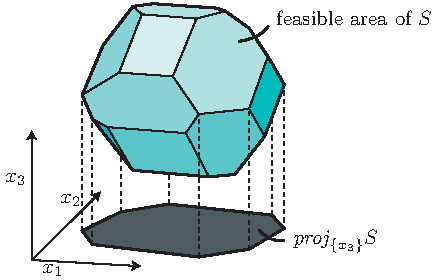
\includegraphics{figures/projection2.pdf}
	\caption{The projection of the system $S$ with respect to $\{x_3\}$.}
	\label{fig:proj}
\end{figure}

The projection of a system $S$ is a set of points in Euclidean space, and it is the feasible region of (another) system $S'$ (see e.g. \cite{ziegler95}). However, many constraint systems determine the same feasible area, and when we say e.g. ``$S'$ is the projection of $S$ w.r.t. $Y$'' we mean that ``$S'$ is one of the constraint systems whose feasible area equals the projection of the feasible area of $S$ w.r.t $Y$''.

In this article, we are mainly interested in the original system $S$ and its projection $S'$, while the associated feasible areas of $S$ and $S'$ are the ``mediator'' between the two systems. However, since the feasible area of a system is just a set of points in a multi-dimensional Euclidean space, the number and the order of the variables are important. To simplify the presentation, though, we do not specify $\VAR(S')$ formally for every considered constraint system $S$. Intuitively, we just make sure that the dimensions (and order of variables) ``match''. For example, when two systems $T$ and $T'$ are joined to form another system $T''$, we consider $T$ and $T'$ as constraints over the same variable set, $\VAR(T'')=\var(T)\cup \var(T')$. A more stringent exposition keeping track of the variable sets and ordering can be found in \cite{MyTechRep}.

\subsection{Projection procedure} \label{sec:methods}
Our projection framework is based on Fourier-Motzkin elimination for calculating the projection of the constraint system $S$ w.r.t. $Y$. It consists of several sub-procedures. The methods for projecting any (not necessarily structured) constraint system are described further below in this section, while the decomposition used on block-angular structured problems will be described in the next section.

Overall, we begin by preprocessing the constraint system, i.e. we reduce it by removing easily identifiable redundant constraints and assign necessary bounds and values to variables (e.g., \cite{brearley75,andersen95,maros}).
Then we use the equalities in the reduced system to isolate variables from $Y$ and substitute in the rest of the system. This eliminates variables from the system, and we refer to it as \emph{Gauss-elimination} (e.g., \cite{duffin74,simon05}).  
Subsequently, we successively eliminate one variable from $Y$ using Fourier-Motzkin elimination and remove redundant inequalities from the system afterwards, until no more variables remain to be eliminated. Eliminating a variable from the system causes some of its constraints to be removed, while new inequalities are added. Only the added inequalities are checked for redundancy since the remaining constraints have already have been checked previously and do not later become redundant. At the top-level, the pseudocode for our projection method is thus as described in the pseudocode below in Algorithm~\ref{alg:FMEF}. 
\begin{algorithm}
\caption{The projection method based on Fourier-Motzkin elimination} 
\label{alg:FMEF}
\begin{algorithmic}
\Function{Project}{System $S$, Variables $Y$}
	\State $(S,Y)\gets \Call{Preprocess}{S,Y}$
	\State $(S,Y)\gets\Call{Gauss-Elim}{S,Y}$
	\While{$Y\neq\emptyset$}
		\State $(S, Y, New )\gets\Call{FME-SingleVar}{S,Y}$
		\State $S\gets\Call{RemoveRedundancy}{S,New}$
	\EndWhile
	\State \Return $S$
\EndFunction
\end{algorithmic}
\end{algorithm}
Each sub-procedure in this algorithm is detailed further below. We start with the methods for variable elimination, before we describe the redundancy removal and finally the preprocessing step. We first describe the two types of eliminations used, namely Fourier-Motzkin-elimination and Gauss-elimination. 

\subsubsection{Fourier-Motzkin-elimination} 
Fourier-Motzkin Elimination (FME) is a classical algorithm for producing the projection of a set of variables from an inequality system, i.e. a constraint system with no equalities. The method successively eliminates one variable $x\in Y$ until all required variables have been eliminated. To eliminate a single variable $x\in Y$ from the constraint system $S$, the constraints are first divided into sets, $\Pos_S(x)$, $\Neg_S(x)$ and $\mi{Zero}_S(x)$ depending on the sign of $x$'s coefficient. Since the method traditionally works on systems without equalities, each equality $e: \ve{a}\cdot\ve{x} = b$ is here treated as two inequalities $\ve{a}\cdot\ve{x} \leq b$ and $-\ve{a}\cdot\ve{x} \leq -b$. Bounds are treated as any other inequalities, so if $ub_x$ is an upper bound for $x$, then $x\leq ub_x$ is added to $\Pos_S(x)$, and if $lb_x$ is a lower bound for $x$, then $-x\leq - lb_x$ is added to $\Neg_x(S)$. A new system $S'$ is then created, which consists of $\mi{Zero}_S(x)$, together with one inequality, $i_{p,n,x}$, for each pair $(p,n)\in \Pos_S(x)\times \Neg_S(x)$. $i_{p,n,x}$ is the addition of positive multiples pf $p$ and $n$ such that the coefficient of $x$ in the resulting inequality is $0$, i.e., if $p$ equals $\ve{a}\cdot\ve{x} \leq b$ and $n$ equals $\ve{a}'\cdot\ve{x} \leq b'$, then $i_{p,n,x}$ is the inequality 
\[
i_{p,n,x}: -a'_x\cdot \ve{a}\cdot\ve{x} + a_x\cdot \ve{a}'\cdot\ve{x} \leq -a'_x\cdot b + a_x\cdot b'.
\]
By construction, the coefficient for $x$ in $i_{p,n,x}$ is zero, and the resulting system $S' = \mi{Zero}_S(x) \cup\\
\set{i_{p,n,x}}{(p,n)\in \Pos_S(x)\times Neg_S(x)}$ is the projection of $S$ w.r.t. $\{x\}$.  

The order in which variables are eliminated naturally influences the size of the intermediary inequality systems. We have chosen to use the greedy heuristic {that minimizes the number of new inequalities in the immediately next system \cite{duffin74}}, which is a commonly used heuristic. It is easily calculated from the current system as the variable $x\in Y$ that minimizes $|\Pos_S(x)||\Neg_S(x)| - |\Pos_S(x)|-|\Neg_S(x)|$.  In the worst case scenario, where $|\Pos_S(x)| = |\Neg_S(x)| = \frac{|S|}{2}$ for all $x\in Y$, the number of inequalities in the created system $S'$ is $\frac{1}{4}|S|^2$, which implies that (both time and space) complexity is double-exponential. For a large, dense system, the growth will be substantial, which prohibits it from use for practical purposes \emph{if} the added inequalities are non-redundant or the non-redundant inequalities are not removed ({see e.g. \cite{lassez93} and \cite{lukatskii08}}). It should, however, also be emphasized that not all inequalities in the succeeding system are necessarily non-redundant; in fact, the number of non-redundant inequalities will at most grow exponentially \cite{monniaux10}.

\subsubsection{Gauss-elimination} 
Equalities in a constraint system can be treated as two inequalities when doing FME as described above. However, an equality $e$ can also be used to isolate a variable $x\in Y$ which can then be substituted in all other constraints in $S$. We refer to this as Gauss-elimination of the variable $x$ using $e$. This also eliminates $x$ from the system and does not cause the same combinatorial explosion of inequalities as FME may do (e.g., \cite{duffin74,simon05}). Before performing FME we therefore do as many Gauss-elimination of variables in $Y$ as possible. To avoid density, when the system $S$ contains several equalities, we first choose the variable $x$ (used in any equality) that is used the fewest times in total in $S$. We then choose the equation $e$ among those using $x$ that uses the fewest variables, and do Gauss-elimination of $x$ using $e$.  This is then repeated until there are no more equalities using variables from $Y$.

\subsubsection{Redundancy removal} 
To detect redundancy, we examine each inequality $c: \ve{a}\cdot \ve{x}\leq b$ in turn and remove it from the system if $\max \ve{a}\cdot \ve{x}$ subject to $S\setminus\{c\}$ is less than or equal to $b$. The property can be checked using an LP solver. Though equalities can be examined this way too, we only examine and remove \underline{in}equalities, since we want to keep the equalities for use in Gauss-elimination. Not all inequalities have to be examined, though. When removing redundancy from $S' = \mi{proj}_{\{x\}}S$ we do not need to check inequalities in $\mi{Zero}_S(x)$; if they were non-redundant before the elimination, they will be non-redundant after.

For large systems, checking all constraints for redundancy is time-consuming. We have therefore implemented a method for redundancy removal that uses several threads in parallel. The method uses a manager to keep track of $k>0$ individual workers who do the actual redundancy checking.
The manager assigns a different inequality to each of the workers, who in parallel each check if their own inequality is redundant w.r.t. their own copy of $S$. When each worker is done, it reports the result back to the manager, and it gets a new inequality to check. If the reported inequality was redundant, the other workers are notified and they remove it from their own copy of the system the next time they check a new inequality. The manager collects a set containing all the reported redundant inequalities, and when all inequalities are checked, these inequalities can then be removed from the system. For the method to work correctly, it is important that $S$ contains no two constraints defining the same halfspace. Such easily detectable redundancies are removed prior to the redundancy removal. We notice that rational numbers are used in the implementation to avid rounding errors. 

Several of the constants in the data used for our vessel models are results of various approximations and hence the boundary of the feasible area is not exact. Coarsening the boundary is therefore permissible, and hence we will also remove inequalities that are \emph{``almost redundant''}. An inequality $c: \ve{a}\cdot\ve{x}\leq b$ is almost redundant if $\max \ve{a}\cdot\ve{x}$  subject to $S\setminus\{c\}$ is less or equal to $b + \epsilon\cdot |b|$ for a small $\epsilon$, see Figure~\ref{fig:almostRedundant}; for our experiments we have used $\epsilon = 0.02$. If $b=0$, we instead require the maximum to be smaller than a given $\epsilon'$. 
\begin{figure}[htbp]
	\centering
		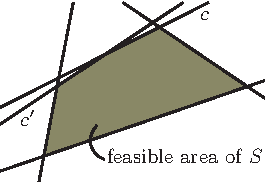
\includegraphics[scale=0.9]{figures/almostRedundant.pdf}
	\caption{The inequality $c$ is almost redundant compared to $c'$, and vice versa.}
	\label{fig:almostRedundant}
\end{figure}
Thus, instead of only collecting a set of redundant inequalities, the manager also collects a set of almost redundant inequalities; the property is checked by the workers simultaneously with the ordinary redundancy check. After the parallel redundancy check, \emph{one} worker then goes through all the almost redundant inequalities one by one and removes the ones that are still almost redundant. The almost redundant inequalities found this way is then removed from the system $S$.  

Notice that almost redundant inequalities can \emph{not} be removed in parallel. Otherwise, in a situation as in Figure~\ref{fig:almostRedundant}, both $c$ and $c'$ could simultaneously be found almost redundant by two different workers, causing them both to be eliminated. When removing almost redundant inequalities sequentially, both inequalities would be checked again, but only the one examined first would be removed. Methods for coarsening the boundary of the feasible area that relies on removing almost redundant inequalities are also used in \cite{lukatskii08} and \cite{shapot12}, though their approaches are different.

\subsubsection{Preprocessing}
Prior to projecting the system, we perform some simple preprocessing steps in order to have a smaller system as the starting point. The steps are then applied repeatedly, as long as a reduction happens in a cycle. A reduction happens if a constraint or variable in $Y$ is removed, a variable is substituted with a value, or a bound of a variable or an (in)equality's left-hand-side is updated. The steps are implemented assuming that the system is feasible.

When performing the preprocessing steps, for each variable $x$, we maintain an upper and lower bound, $ub_x$ and $lb_x$, which initially is $+\infty$ and $-\infty$, respectively. When the bounds are finite, they are treated as inequalities in the system. For each constraint $c$, we likewise maintain an upper and lower bound, $ub_c$ and $lb_c$ for its left-hand-side {based on the bounds of the used variables}. That is, for the inequality $c$ with left-hand-side $\ve{a}\cdot\ve{x}$, we define $ub_c = \smashoperator[r]{\sum_{x. a_x>0}}a_x\cdot ub_x + \smashoperator[r]{\sum_{x.a_x<0}}a_x\cdot lb_x$ and $lb_c = \smashoperator[r]{\sum_{x. a_x>0}}a_x\cdot lb_x + \smashoperator[r]{\sum_{x.a_x<0}}a_x\cdot ub_x$. 
This links the bounds of variables and constraints, and thus, tightening a bound of a variable or constraint can imply a tightening of another bound of a variable or constraint. The individual preprocessing steps are as follows (details can be found in \cite{MyTechRep}). 
\begin{enumerate} \itemsep0em
	\item Remove all empty inequalities and unused variables $x\in Y$.
%
	\item If $ub_x = lb_x$ for a variable $x\in X$, then substitute $x$ with $lb_x$ in all constraints in $S$. 
%
	\item If an inequality $a_x\cdot x \leq b$ belongs to $S$, then remove it from $S$ and update the appropriate bound: If $a_x>0$, update $ub_x$ to $\min\{ub_x,\frac{b}{a_x}\}$, otherwise update $lb_x$ to $\max\{lb_x,\frac{b}{a_x}\}$.
For the equality $a\cdot x = b$, both bounds are updated.
%
	\item If $\Neg_S(x)=\emptyset$ for an $x\in Y$ (implying that $x$ does not occur in an equality and has no (finite) lower bound) then remove $\Pos_S(x)$ from $S$. If $\Neg_S(x)$ only consist of the inequality defining the lower bound of $x$, $-x\leq -lb_x$, then substitute $x$ with $lb_x$ in all constraints in $S$. Similarly w.r.t. $\Pos_S(x)$. We notice that this is \emph{not} a normal preprocessing step, but corresponds to making a FME on $x$, which changes the feasible area of $S$. 
%
	\item Assume $c$ is a constraint with right-hand-side $b$. If ${ub}_c \leq b$, it is redundant and removed if it is an inequality and otherwise (if it is an equality), then necessarily ${ub}_c = b$, and $c$ is removed from $S$ while all positive (respectively negative) variables in $c$ are replaced with their upper (respectively lower) bound.
If $\mi{lb}_c \geq b$, then necessarily $\mi{lb}_c = b$, and $c$ is removed from $S$ while all positive (respectively negative) variables in $c$ are replaced with their lower (respectively upper) bound.
%
	\item For any variable $x$ used by $c$, if $a_x > 0$ and $\mi{lb}_{c,x}<+\infty$, 
	where $\mi{lb}_{c,x} = \smashoperator[r]{\sum_{x'.a_{x'}>0, x'\neq x}}a_{x'}\cdot lb_{x'} + \smashoperator[r]{\sum_{x'.a_{x'}<0}}a_{x'}\cdot ub_{x'}$, 
	then $ub_x$ is updated to $\min\{ub_x, \frac{b-\mathit{lb}_{c,x}}{a_x}\}$. 
	Similarly, if $a_x < 0$ and $\mi{lb}_{c,x}<+\infty$, then $lb_x$ is updated to $\max\{lb_x, \frac{b-\mathit{lb}_{c,x}}{a_x}\}$.	
	Updating bounds for constraints with only one variable (step 3) is a special case of this.
\setcounter{counterName}{\value{enumi}}
\end{enumerate}	
%
Comparing two inequalities syntactically, we can in some cases detect redundancy as described below. All pairs of inequalites are then compared in an efficient manner.
In the following, let $c$ be an constraint in $S$ with left-hand-side $\ve{a}\cdot \ve{x}$ and right-hand-side $b$, and let $c'$ be another constraint with left-hand-side $\ve{a}'\cdot \ve{x}$ and right-hand-side $b'$. 
\begin{enumerate} \itemsep0em
\setcounter{enumi}{\value{counterName}}
\item 
If $\ve{a}=\sigma\cdot \ve{a}'$, then $c$ is \emph{linearly dependent} (\cite{lassez93}). $c$ is hence redundant if
it is an \underline{in}equality and $\sigma\cdot b'\leq b$ and either: $\sigma\geq 0$; or $\sigma<0$ and $c'$ is an equality. $c$ is also redundant if both $c$ and $c'$ are equalities and $\sigma\cdot b'\leq b$. 
It is enough to check if this holds for $\sigma = \frac{c_x}{c'_x}$ for the first variable $x$ used by $c'$.
\item
If all variables used in $c$ and $c'$ are non-negative, and there exists a $\sigma\geq 0$ such that $a_x \leq \sigma \cdot a'_x$ for all $x$, while $\sigma\cdot b' \leq b$, then $c$ is \emph{less strict} than $c'$; it is redundant and hence removed. If $c$ is an equality, so must $c'$ be, and hence $c'$ is turned into an equality. 
This is only required to be tested for specific values of $\sigma$ that depends on whether $c'$ has a variable with a negative coefficient or not \cite{MyTechRep}.
\end{enumerate} 

\subsection{Decomposing block-angular structured system}
\label{sec:decomp}
In the following we will describe how the structure of the considered system can be exploited to make our projection framework scale. Detailed pseudocode and correctness proofs can be found in \cite{MyTechRep}. 

The considered VSMs have a \emph{(primal) block angular structure} \cite{williams}. That is, the constraint system $S$ can be divided into $k$ local subsystems, $S_1, \ldots, S_k$, using smaller, disjoint sets of variables, $X_1, \ldots, X_k$, and a global system, $S_\trt{g}$, whose constraints ``connect'' the otherwise independent subsystem by using variables from several local subsystems (see Figure~\ref{fig:decomp}). 
If there were no global constraints, each subsystem could be projected separately and the resulting systems could then be combined to give the projection of the original system. The global constraints cause the local subsystems to get ``mixed'' when variables are eliminated and hence result in an increasing number of global and dense constraints, which again makes FME perform worse. However, we can still exploit the structure of the problem. We will define and use auxiliary variables to ensure that we can project the subsystems separately without producing global constraints, before we combine the projected subsystems and eliminate the auxiliary variables. To separate and remove local variables from the global constraints, we do as follows for all subsystems $S_i$:
\begin{itemize}\itemsep0em
\item For each global constraint $c$ using variables in $S_i$, we define an auxiliary variable $z^0_{c,i}$ that equals the variables in $S_i$'s contribution to $c$. We add the equality defining $z^0_{c,i}$ to $S_i$, and we substitute with $z^0_{c,i}$ in $c$. For example, if $c: a_1x_1 + a_2x_2 + a_3x_3 + \ldots + a_kx_k \leq b$ is an inequality in $S_\trt{g}$ and $X_i = \{x_1,x_2\}$, then we add $-z^0_{c,i} + a_1x_1 + a_2x_2 = 0$ to $S_i$ and rephrase $c$ as $z^0_{c,i} + a_3x_3 + \ldots + a_kx_k \leq b$. We name the thusly produced subsystem $S_i^0$. 

\item Then, we project $S_i^0$ w.r.t. all variables from $Y$ that are present in $S_i^0$. We do keep the auxiliary $z^0$-variables. 
Because of these auxiliary variables this only produces inequalities with variables not present in other subsystems $S_j$. 
\end{itemize}
After projecting each $S_i^0$ we can then combine the results with the rephrased, global constraints, $S_\trt{g}^0$, to create the system $\mathcal{S}$, i.e. 
\begin{equation}\label{eq:curlyS}
\mathcal{S} = S^0_\trt{g} \cup S'^0_1\cup \ldots \cup S'^0_k,
\end{equation}
where $S'^0_i$ is the projection of $S^0_i$ w.r.t. $Y\cap X_i$ for all $i\in\{1,\ldots, k\}$.
We can then eliminate all the auxiliary $z^0$-variables, $Z^0$, plus the variables in $Y$ not occurring in any $S_i$ from $\mathcal{S}$. 
\begin{figure}[htbp]
	\centering
		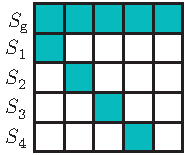
\includegraphics{figures/blockStructure.pdf}
	\caption{An illustration of the coefficient matrix for a block-angular constraint system $S$ (non-zero sections coloured blue).}
	\label{fig:decomp}
\end{figure}

\paragraph{Example}
As an example, consider the block-structured (in)equality system $S = S_\trt{g} \cup S_1\cup S_2\cup S_3 \cup S_4$ below, which is illustrated in Figure~\ref{fig:decomp}. 
\small{
\begin{gather*}
S_\trt{g}: \left\{ \begin{array}{lrl} e:& -u + x_1 + y_1 + 2 x_2 + 2 y_2 + 3 x_3 + 3 y_3 + 4 x_4 + 4 y_4 &= 0\\
c:& x_1 + 2 y_1 + 3 x_2 + 4 y_2 + 5x_3 + 6 y_3 + 7x_4 + 8 y_4 &\leq 16\end{array}\right.,\\ 
S_1: \left\{ \begin{array}{ll}x_1 + y_1 				&\leq 5\\
															x_1 - 3 y_1 &\leq 1\\
														4 x_1	+ 2 y_1 	&\leq -1\end{array}\right.,\qquad
S_2 : \left\{ \begin{array}{ll}  x_2 - 2 y_2 &\leq 2\\
															 - x_2 - y_2 				&\leq -2\\
																 y_2 							&\leq 4\end{array}\right.,\qquad
S_3 : \left\{ \begin{array}{ll}- x_3 + y_3 			&\leq 3\\
														 - 2 x_3 - y_3 			&\leq -1\\
																 x_3 						&\leq 4\end{array}\right.,\quad
S_4 : \left\{ \begin{array}{ll} x_4 +2 y_4 &\leq 8\\
															- x_4 						&\leq -1\\
															- y_4 						&\leq -1\end{array}\right..
\end{gather*}
}
\normalsize{
Assume that we want to eliminate all variables but $u$, which is defined as a weighted sum of the rest of the variables.
We then define $S_\trt{g}^0, S_1^0, S_2^0, S_3^0$ and $S_0^4$ as below. Then we project each $S_i^0$ w.r.t. $\{x_i, y_i\}$, join the projections together with $S^0_\trt{g}$ in the system $\mathcal{S}$, and then project $\mathcal{S}$ w.r.t. $\{z^0_{e,1}, z^0_{e,2}, z^0_{e,3}, z^0_{e,4}, z^0_{c,1}, z^0_{c,2}, z^0_{c,3}, z^0_{c,4}\}$.}
\small{
\begin{gather*}
S_\trt{g}^0 = \{-u + z_{e,1}^0 + z_{e,2}^0 + z_{e,3}^0 + z_{e,4}^0 = 0, \: 
z_{c,1}^0 + z_{c,2}^0 + z_{c,3}^0 + z_{c,4}^0 \leq 16\},\\
S_1^0 = S_1\cup \{-z_{e,1}^0 + x_1 + y_1 = 0,\: -z_{c,1}^0 + x_1 + 2 y_1 = 0 \},\quad
S_2^0 = S_2\cup \{-z_{e,2}^0 + 2 x_1 + 2 y_1 = 0,\: -z_{c,2}^0 + 3x_2 + 4 y_2 = 0 \},\\
S_3^0 = S_3\cup \{-z_{e,3}^0 + 3 x_1 + 3 y_1 = 0,\: -z_{c,3}^0 + 5 x_3 + 6y_3 = 0 \},\quad
S_4^0 = S_4\cup \{-z_{e,4}^0 + 4 x_1 + 4 y_1 = 0,\: -z_{c,4}^0 + 7 x_4 + 8y_4 = 0 \}.
\end{gather*}
}

\normalsize{Comparing the union of the new (unprojected) subsystems, $\mathfrak{S} = S_1^0\cup\ldots\cup S_k^0\cup S_\trt{g}^0$, with the original system $S$, all we have done is defining auxiliary variables and substituted them in the system. Thus, eliminating the variables in $Y$ from $S$ is equivalent to eliminating $Y$ and the defined $z^0$-variables from $\mathfrak{S}$.} This, in turn, is equivalent to projecting the subsystems $S^0_i$ separately w.r.t. $X_i\cap Y$, combining the resulting systems with $S^0_\trt{g}$, and then eliminate the $z^0$-variables and the remaining $Y$-variables: % The intuition behind this is, as follows: 
%
When eliminating $Y\cup Z^0$ from $\mathfrak{S}$, we can choose to first eliminate $X_1\cap Y$, then $X_2\cap Y$ up to $X_k\cap Y$, and finally $Z^0\cup Y\setminus(X_1\cup \ldots\cup X_k)$. 
Any variable in $X_1\cap Y$ has a zero-coefficient in all constraints not in $S^0_1$, and the constraints in $\mathfrak{S}\setminus S^0_1$ will therefore not be changed by the FME procedure when the variables in $X_1\cap Y$ are eliminated.  We can therefore set aside these inequalities until we have eliminated all variables in $X_1\cap Y$. Likewise, when eliminating variables in $X_i\cap Y$, no constraint from either $S_{i+1}^0\cup \ldots \cup S_k^0\cup S_\trt{g}^0$ or the already projected systems contain any variables from $X_i\cap Y$ and can hence be put aside and only included later when the variables in $Z^0\cup Y\setminus(X_1\cup \ldots\cup X_k)$ are eliminated. Thus, the following holds. 
\begin{prop}
{The projection of $S$ w.r.t. $Y$ defines the same feasible area as 
the projection of $\mathcal{S}$ w.r.t. $Z^0 \cup Y\setminus (X_1\cup \ldots \cup X_k)$, where
$\mathcal{S}$ is as defined in \eqref{eq:curlyS}.% = S^0_\trt{g} \cup S'^0_1\cup \ldots \cup S'^0_k$ and $S'^0_i$ is the projection of $S^0_i$ w.r.t. $Y\cap X_i$ for all $i\in\{1,\ldots, k\}$.
}
\end{prop}

$\mathcal{S}$ has by construction a block-angular structure and instead of eliminating $Z^0\cup Y\setminus(X_1\cup\ldots\cup X_k)$ immediately, if necessary, we can use further auxiliary variables to postpone ``mixing'' blocks when eliminating the remaining variables. 
To do so, we collect all subsystems into $k_1$ small groups; we have mostly used groups of size 2, 3 or 1\footnote{``Combining'' a single subsystem corresponds to substituting a variable with a new variable, but can be done for convenience of notation.}. For each group $i$ we do as follows:
\begin{itemize}\itemsep0em
\item We join the systems in the group into a new system, $S^1_i$. For each (rephrased) global inequality $c$ using variables occurring in $S^1_i$, we then define a variable, $z^1_{c,i}$, that equals $S^1_i$'s contribution to $c$. We then add the defining equality to $S^1_i$ and rephrase $c$ using $z^1_{c,i}$.
\item Then we project the resulting system, $S^1_i$, w.r.t. the previous, auxiliary $z^0$-variables, while we keep the newly created $z^1$-variables.
\end{itemize} 
Subsequently we can then join the projected $S^1$-systems with the (rephrased) transverse inequalities, $S_\trt{g}^1$, and finally project the last auxiliary variables. Alternatively, we can repeat the steps above until the final projection can be done. 

Each time we further decompose a system, we use a partitioning of the subsystems $S^l_1, \ldots, S^l_{k_l}$ to create a new level of $k_{l+1}$ subsystems, $S^{l+1}_1,\ldots, S^{l+1}_{k_{l+1}}$. This effectively creates a tree structure of smaller inequality systems, where each node is associated with a subsystem and a set of variables that should be eliminated from the system. Using this tree, an inequality system associated with a node is projected by recursively projecting the systems associated with the children of the node. Further, as expected, projecting the root of the tree constructed from $S$ and $Y$ creates a system equivalent to the projection of $S$ w.r.t. $Y$. See Figure~\ref{fig:decomp2} and the example further below.

\begin{figure}[htbp]
	\centering
		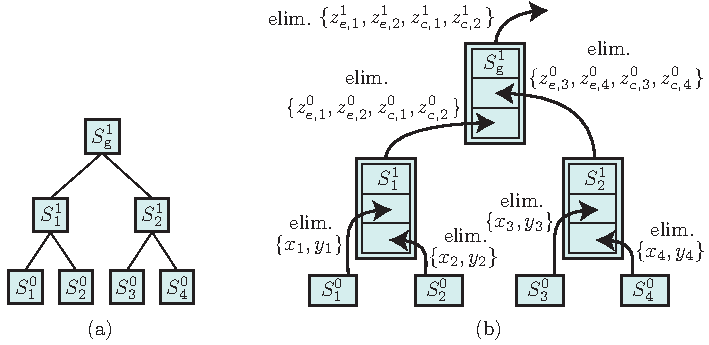
\includegraphics{figures/Example3.pdf}
	\caption{(a) A system $S$ decomposed into a tree structure of subsystems. (b) Recursive projection of the tree-structure in (a).}
	\label{fig:decomp2}
\end{figure}

The intuition why this works is as before; projecting all $Y$ and $Z$-variables from the union of all the (unprojected) subsystems in the nodes of the tree corresponds to projecting the $Y$ variables from $S$, and because we can choose the elimination order of the variables, we only need to project the subsystems in the tree in the correct order (a rigorous proof can be found in \cite{MyTechRep}).

\begin{prop}
The projection of the system associated with the root of the tree constructed from $S$ and $Y$ w.r.t. the $Y$- and $Z$-variables as described corresponds to projecting $S$ w.r.t. $Y$.
\end{prop}

\paragraph{Example}
Consider the system from the previous example, which was decomposed into the subsystems $S^0_1, S_2^0, S_3^0, S^0_4$ and $S^0_\trt{g}$. Instead of projecting these subsystems as described in the previous example, we insert an additional level in the decomposition. We group the four subsystems into two groups, $\{S^0_1, S^0_2\}$ and $\{S^0_3, S^0_4\}$, and construct the tree structure in Figure~\ref{fig:decomp2}(a), where 
\small{\begin{gather*}
S_\trt{g}^1 = \{-u + z^1_{e,1} + z^1_{e,2} = 0,\: z^1_{c,1} + z^1_{c,2} \leq 16 \},\\   
S^1_1=\{-z^1_{e,1} + z^0_{e,1} + z^0_{e,2} = 0,\: -z^1_{c,1} + z^0_{c,1} + z^0_{c,2} = 0\}, 
\quad S^1_2=\{-z^1_{e,2} +z^0_{e,3}+ z^0_{e,4} = 0,\: -z^1_{c,2} +z^0_{c,3}+ z^0_{c,4} = 0\}. 
\end{gather*}}
\normalsize{The projection of $S$ w.r.t. $\{x_1,y_1,x_2,y_2,x_3,y_3,x_4,y_4\}$ is now made by projecting the root of the tree recursively as shown in Figure~\ref{fig:decomp2}(b).}

%\subsubsection{Projection via decomposition}
Using our previously described projection method, we obtain the projection of $S$ w.r.t. $Y$ by calling \Call{ProjectNode}{root of $T$}, where $T$ is the tree structure constructed from $S$ and $Y$, and \Call{ProjectNode}{} is as below in Algorithm~\ref{alg:decomp}. We note that due to the boundary coarsening (elimination of almost redundant inequalities), this only approximates $\mi{proj}_Y(S)$. However, by setting $\epsilon = 0$, the algorithm indeed returns the correct projection.

\begin{algorithm}
\caption{{Projecting a block-angular structured system using decomposition.}}
\label{alg:decomp}
\begin{algorithmic}
\Function{ProjectNode}{Node $n$} 
	\State $(S,Y)\gets$ the system and variable set associated with $n$
	\If{$n$ is a leaf}
		\State \Return \Call{Project}{$S$, $Y$}\Comment Algorithm~\ref{alg:FMEF}
	\Else
		\ForAll{children $m$ of $n$}
			\State $S \gets S\cup \Call{ProjectNode}{m}$ 
		\EndFor
		\State \Return $\Call{Project}{S, Y}$ \Comment Algorithm~\ref{alg:FMEF}
	\EndIf
\EndFunction
\end{algorithmic}
\end{algorithm}
%
%\paragraph{{Other block structures} }

\noindent Using the decomposition described above, it is of course also possible to project nested block structured problems, i.e. systems that on the top-level can be divided into a global part and a number of local parts that in themselves can be further divided into local parts and a global part, and so on.  
Other block structured problems such as staircase problems can also be decomposed into a tree structure and projected using the described approach. 
\\\\
%\paragraph{\red{Parallelization}}
When the system $S$ is decomposed into subsystems in a tree structure as described above, the projection itself can be parallelized by maintaining a queue of not yet projected subsystems whose children have all been projected; this queue thus initially contains all leafs. 
The members of the queue are then solved independently by multiple solvers in parallel, who also add systems to the queue when the membership condition is met.
The pseudocode for this is presented below. Besides a system $S$ and a variable set $Y$, each node $n$ is associated with a number, $n_{count}$, corresponding to the number of projected children (initially set to $0$), and a system, $n_{proj}$, corresponding to the projection $\mi{proj}_Y(S)$ when it is done (initially set to $\emptyset$). 
\vspace{1mm}

\begin{algorithmic}
\Function{ParallelTreeProjection}{$S$, $Y$}
	\State Construct  tree structure $T$ from $S$ and $Y$
	\State $n_{count}\gets 0$ and $n_{proj}\gets\emptyset$ for all nodes $n$ in $T$
	\State Create a set $W$ of workers, initially idle
	\State Initialize a queue $Q$ with all leaves in $T$
	\While{$\mi{root}(T)_{proj} = \emptyset$}
		\If{$Q$ is non-empty and a worker $w\in W$ is idle}
			\State Remove first node $n$ from $Q$
			\State Use $w$ to call \Call{ProjectSingleNode}{$n$}
		\EndIf
	\EndWhile
	\State \Return $\mi{root}(T)_{proj}$
\EndFunction
\Statex
\Function{ProjectSingleNode}{Node $n$}
	\State $(S',Y')\gets$ the system and the variable set associated with $n$
	\State $S'\gets S'\cup_{m\in \mi{children}(n)} m_{proj}$ 
	\State $n_{proj}\gets$ \Call{Project}{$S'$,$Y'$} \Comment Algorithm~\ref{alg:FMEF}
	\State $\mi{parent}(n)_{count} \gets \mi{parent}(n)_{count} +1$
	\If{$\mi{parent}(n)_{count} = |\mi{children}(\mi{parent}(n))|$}
		\State Add $\mi{parent}(n)$ to $Q$
	\EndIf
	\State \Return
\EndFunction
\end{algorithmic}	

\vspace{1mm}
All workers project a system using the FME framework, which again involves parallel redundancy removal, and thus it is important to only use as many resources (threads) in total as there are available.
Then, when at some point there are less nodes left to project than there are workers in $W$, the superfluous workers can pass on their resources to the remaining workers.  

\section{Results}\label{sec:results}
We have constructed a number of different VSMs from data for a specific vessel, where the weight and hydrostatics are taken into account to various degrees. The first VSM does not consider the weight of the containers at all (i.e. the described constraints limiting the total displacement as well as all hydrostatic constraints have been removed), the second VSM does not model any hydrostatic constraints, and the subsequent VSMs consider the hydrostatic constraints at 2, 4, 6 and 8 measure points, respectively.

Each VSM has been transformed into its corresponding VCM. That is, all variables but $\set{x_\tau}{\tau\in T}$ have been eliminated. Projections have been done in two different ways, decomposed and flat. For the decomposed projections, a tree structure has been used as described in the previous section, while the flat projections do not use any decomposition at all. 
Our FME-based projection framework has been implemented in Java. The experiments were carried out on a computer with an {Intel\textsuperscript{\textregistered} Xeon\textsuperscript{\textregistered} E5-1660 V4 processor with a frequency of 3.20-3.80 GHz, 32GB RAM, and with 8 cores and 16 threads.}

The VSMs and VCMs have been optimized for revenue. The optimal objective value as well as time taken has been compared. The latter is measured in both iterations and \emph{ticks} as it appears when solved with CPLEX Interactive Optimizer version 12.5.0.0. Ticks is a deterministic time measure that according to the software provider ``yields the same level of performance for repeated solving of the same model with the same parameter settings, on the same computing platform''. The revenue is dependent on the container type, so that the container types that (in the industry) are found more limiting also yields a higher revenue, see further below. 

\subsection{Size reduction}
Table~\ref{tab:projections} summarizes the size of the original (unprojected) VSMs and the VCMs that are the result of the projection using decomposition. These sizes are given in terms of the number of inequalities (ineqs), variables (vars), non-zero entries (nzs.) and density (dens.). The size of the original models are given both as they appear as input to our algorithm, but also after a {competitive} preprocessing, namely after it has been preprocessed by CPLEX. For comparison, the table includes the simple VCM for the particular vessel, we have used. This VCM is the one currently used in the industry, and it only includes upper bounds on the total number of containers, the total number of reefer containers, and the total weight.  

\begin{table}[htbp]
\centering
\begin{tabular}{l|r@{ / }r@{ / }r@{ / }r|r@{ / }r@{ / }l@{ / }r|r@{ / }r@{ / }r@{ / }r}
\toprule
$\multirow{2}{*}{Model}$&\multicolumn{4}{c|}{VSM size}&\multicolumn{4}{c|}{VSM, presolved}& \multicolumn{4}{c}{VCM size}\\
&ineqs (eqs)&vars&nzs.& dens.&rows&cols&nzs.&dens.&ineqs&vars&nzs.&dens.\\
\midrule
{No weights} &774 (12)&1142&6662&8.61&	554&657&2784&5.03&				20&12&\phantom{1}155&7.75\\  
{No hydro.} &806 (43)&1173&7854&9.74&	555&657&3441&6.20&		18&12&\phantom{1}144&8.00 \\ 
{2 parts} &810 (43)&1173&7860&9.70&	556&661&3447&6.20&					96&12&1113&11.59\\ 
{4 parts} &824 (49)&1179&7886&9.57&	564&671&3471&6.15&	64&12&\phantom{1}731&11.42\\
{6 parts} &838 (55)&1185&7916&9.44&	570&679&3496&6.13&	80&12&\phantom{1}888&11.10\\
{8 parts} &852 (61) &1191 &7950&9.33	&	576&685&3522&6.11&	52 &12&\phantom{1}582&11.19\\
\bottomrule
\multicolumn{10}{c}{}\\
\cmidrule{1-9}
Simple VCM & 3&12 &\phantom{12}36&12.00&3&9&\phantom{12}24&\multicolumn{1}{l}{8.00}\\
\cmidrule{1-9}
\end{tabular}
\caption{The size of the VSMs, before and after projection into VCMs, given in terms of the number of inequalities (ineqs), variables (vars), non-zero entries (nzs.), and density (dens.) The size of the simple VCM is included for comparison. }
\label{tab:projections}
\end{table}
The results show that the VCMs have much fewer inequalities and variables, namely app. 6 - 30 times fewer inequalities and 54-57 times fewer variables than even the presolved VSMs. The VCMs also have fewer non-zero entries (between 3 and 24 times fewer), though, the VCMs are more dense (app. 1.3 to 1.9 more dense than the presolved VSMs). The results reveal no apparent relationship between the size of the VSM and the size of its VCM. This may have to do with both the actual position of the hydrostatic measure points and the non-deterministic behaviour of the removal of almost redundant inequalities. 

\subsection{Decomposition impact}
Table~\ref{tab:time} shows the time taken for the algorithm to do the projection, both decomposed and flat. For most VSMs, the flat projection timed out (TO) after 65 hours, in which case the variables left to be projected are given. Figure~\ref{fig:8parts} shows the progression of the number of inequalities and variables, respectively, as a function of time when the algorithm runs on the decomposed 8 part-model. These numbers are the sum of all the inequalities and variables, respectively, in all the projected or unprojected subsystems in the decomposition at a given time. Likewise, Figure~\ref{fig:compare} shows the progression for the flat projection of the same model; this figure includes the number of inequalities for the decomposed projection for comparison. Each graph shows the number of inequalities and variables after the preprocessing step, each Gauss-elimination, and each FM-elimination followed by some preprocessing, parallel redundancy removal and sequential removal of almost redundant inequalities.    
\begin{table}[htbp]
\centering
\begin{tabular}{l|r@{\hspace{-3em}}rc|rc}
\toprule
$\multirow{2}{*}{Model}$&\multicolumn{5}{c}{Time}\\
&\multicolumn{2}{r}{decomp.}& vars left to project&flat&vars left to project\\
\midrule
{No weights}& &24.5m&-&2.5m&-\\
{No hydro.}& &14.5m&-&1.8m&-\\
{2 parts} &7h&18m &-&(TO) 32h& 551\\
{4 parts} &8h&4m &-&(TO) 61h & 557\\
{6 parts} &3h&7m &-&(TO) 18h & 577\\
{8 parts} &3h&19m &-&(TO) 65h& 566\\
\bottomrule
\end{tabular}
\caption{Time taken to do the projections, using decomposition or not (flat), respectively. The time limit is set to 65 hours.}
\label{tab:time}
\end{table}

The results in Table~\ref{tab:time} shows that the decomposition has a substantial impact on the success of the projection algorithm when the VSM includes hydrostatic constraints. The table also shows that the two smallest VSMs that do not take hydrostatic constraints into consideration are solved faster using a flat projection. This behaviour is not surprising, since the hydrostatic constraints are dense, global constraints that links the weight of all sections to the left or right of a measure point, and the coefficients in the constraints are non-trivial. Thus, when these are included, decomposition is useful while not necessary for the simpler systems.
 
\begin{figure}[htbp]
	\centering
		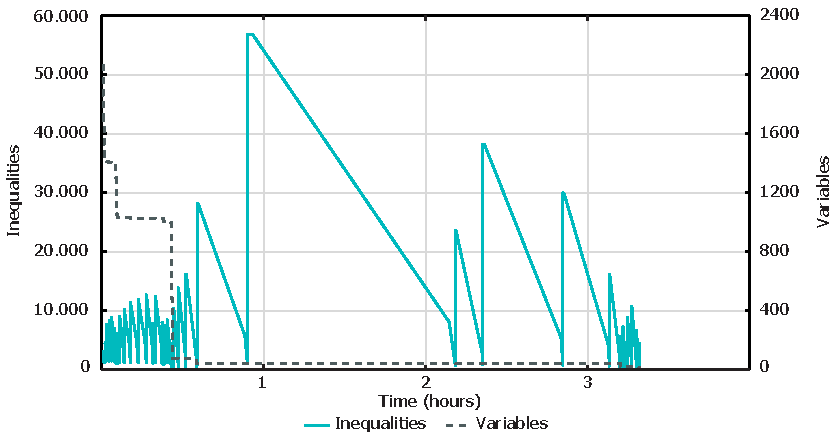
\includegraphics[scale=0.7]{figures/decompIneqGrowth2.pdf}
	\caption{The inequalities growth and variable decrease for the 8 part-model with decomposition.}
	\label{fig:8parts}
\end{figure}

\begin{figure}[htbp]
	\centering
		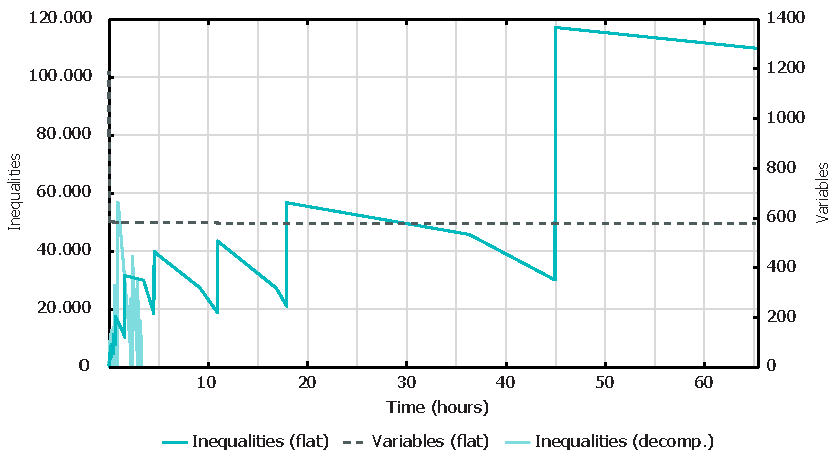
\includegraphics[scale =0.7]{figures/ineqGrowth2.pdf}
	\caption{The inequalities growth for the 8 part-model with and without decomposition.}
	\label{fig:compare}
\end{figure}

When considering each subsystem in a decomposition as a system in itself, in general, the number of inequalities after each call to \Call{FME-SingleVar}{} in Algorithm~\ref{alg:FMEF} grows to begin with, as does the number of inequalities before this call. This continues until there are a few variables left, where both these numbers decrease. Notice, that the graph in Figure~\ref{fig:8parts} shows the total run of the projection algorithm, causing this pattern to be repeated. Hence it may be hard to see this in the figure.

For the decomposed algorithm, though the number of inequalities grow after each FME-step, most of them are redundant or almost redundant. The same does not hold for the flat projection for the cases where hydrostatics are taken into consideration, at least not for the FME-steps that are completed within the time limit. Instead, many of the produced inequalities are non-redundant which increases the likelyhood that even more inequalities will be produced in the next elimination, but also that the redundancy removal will take longer time - not only are there more inequalities to check, each check will also take longer. Though this is just speculations, since the flat projections were not finished due to time and memory constraints, it appears that the flat projection of the total system on a ``global'' scale behaves as an ``enlarged'' version of described pattern for the subsystems.
This behavior can be explained by the occurrence of several ``interacting'' global constraints: the algorithm projects a few variables from one subsystem (resulting in a little denser global constraints) before moving on to the next subsystem from where it removes another few variables etc., all the while it postpones dealing with the variables in the global inequalities which get more and more dense. It should be mentioned that it is possible, that other orderings of the variables (caused by other heuristics than the used greedy heuristic) in these cases could potentially lead to manageable flat projections, but testing this is outside the scope of this paper.  
We also note that the runtime, even for the decomposed projections, are not exactly small, and the main part of the execution time is spend doing redundancy removal. However, as mentioned in the introduction, these calculations are off-line that should be done once, after which they can be used as submodels in other optimization models.  

\subsection{Revenue optimization}
The VSMs and their projected VCMs have been optimized for revenue using CPLEX. Each transported container yields a revenue based on its type, i.e. on the size, weight and reefer-property of the container. More specifically, for our tests, reefer containers yield the double revenue of a similar non-reefer container, $40'$ containers have a revenue which is 1.5 times higher as a similar $20'$ container, while containers are more expensive the heavier it is. A $20'$, non-reefer container, with a weight, respectively of 6, 21, and 27 ton, is assigned the following revenue in USD: 100, 600 and 700, respectively. Table~\ref{tab:usingProjections} shows the number of iterations, the deterministic time and the optimal objective value found by CPLEX when optimizing revenue for the VSMs and projected VCMs. It likewise shows how many times faster, the projections are w.r.t. iteration and ticks, as well as the difference in optimal objective value in percentage. For comparison, the number of iterations, deterministic time and objective value is shown too for the simple VCM.
\begin{table}[htbp]
\centering
\begin{tabular}{l|rrr|rrr|rrr}
\toprule
Model&\multicolumn{3}{c|}{VCM}&\multicolumn{3}{c|}{VSM}&\multicolumn{3}{c}{Difference}\\
&Iter.&Ticks&Objective&Iter.&Ticks&Objective&Iter. (times)&Ticks (times)&Obj. (\%)\\ 
\midrule
No weights&	11 & 0.05 & $8.63\cdot 10^6$ &	363 & 2.64&$8.08\cdot 10^6$
&33.0&52.8&6.8\\
\midrule
{No hydro.}& 9 & 0.04 &$7.87\cdot 10^6$&	188 & 5.48&$6.22 \cdot 10^6$
&20.9&137&26.5\\
\midrule
{2 parts}& 14 & 0.29 & $6.09\cdot 10^6$ &	251 & 5.88&$6.07\cdot 10^6$
&17.9&20.3&0.196\\
\midrule
{4 parts} &13 & 0.18 &$6.17\cdot 10^6$ & 228 & 4.95 &$6.16\cdot 10^6$
&17.5&27.5&0.153\\
\midrule
{6 parts} &9 & 0.20& $6.17\cdot 10^6$ &227 & 5.02 &$6.18\cdot 10^6$
&25.2&25.1&0.202\\
\midrule
{8 parts} &12 & 0.14& $6.21\cdot 10^6$ & 233 & 4.79 &$6.18\cdot 10^6$
&19.4&34.2&0.490\\
\bottomrule
\multicolumn{10}{c}{}\\
\cmidrule{1-4}
Simple VCM & 4 & 0.02 &\multicolumn{2}{l}{$1.07\cdot 10^7$}\\
\cmidrule{1-4}
\end{tabular}
\caption{Iterations, time and objective values for VCMs and their unprojected VSMs, as well as for the simple VCM. }
\label{tab:usingProjections}
\end{table}

As can be seen from the numbers in Table~\ref{tab:usingProjections}, in general, VCMs are much faster to solve than their corresponding VSMs. More specifically there are between approx. 17 and 33 times fewer iterations and 20-137 times fewer ticks, which corresponds to a difference between 94\% and 97\% of the number of iterations, and 96\% and 99.5\% CPLEX ticks, respectively. Meanwhile the difference in objective value is only modest; for the models including hydrostatic constraints, the difference is at most 0.5 \%, while the other two models have a difference of 6.8 and 26.5 \%, respectively. 
When comparing to the simple model, we see that this model of course is even faster (between 41-97 times (iterations) and 132-294 (ticks)), but the difference in objective is also between 72\% and 76\% for the last 5 models. Hence, our results confirm the experiments by Delgado \cite{AlbertosThesis} showing a substantial revenue overestimation when using the simple model. 

\subsection{Projection of multi-commodity flow problems}
Beside the VSM, we have studied another block-angular structured system, namely one describing a multi-commodity flow problem. In a multi-commodity flow graph $G=(V,E)$ with $k$ commodities, we have a positive variable $x_{e,i}$ for each edge $e\in E$ and commodity $1\leq i\leq k$, which denotes the number of goods of commodity $i$ that flows on the edge $e$. There is an upper bound on each $x_{e,i}$ as well as a common upper bound for the sum of commodities on an edge. 
Supply and demand are modeled with variables $x_e,i$ for (artificial) edges going to source nodes (from nowhere), $\mi{ES}_G$, and edges going from sinks (to nowhere), $\mi{ET}_G$, respectively. 
Constraints ensure that for all commodities $i$ and all nodes $n$ %-- except for source nodes $S\subseteq V$ and sink nodes $T\subseteq V$ -- that
the sum of goods of commodity $i$ on edges going to $n$ equals the sum of good of commodity $i$ on edges going away from $n$. Considering the case, where demands and supply are not given, we want to know how the amount of each commodity at the sinks depends on the amount of each commodity at the sources. Therefore we eliminate all variables $x_{e,i}$, where $e\notin \mi{ES}_G\cup \mi{ET}_G$, from the constraint system describing the flow problem. 

A multi-commodity flow problem is naturally block-structured, though, there are usually many global constraints -- corresponding to the common upper limits for each edge. Instead of using these blocks to decompose the system, it is also possible to divide the graph into smaller subgraphs. We then treat the ingoing edges in a subgraph $G'$ as supply edges ($\mi{ES}_{G'}$) and the outgoing edges as demand edges ($\mi{ET}_{G'}$), and eliminate all variables but $\{\;x_{e,i}\;|\; e\in \mi{ES}_{G'}\cup \mi{ET}_{G'}, 1\leq i\leq k\;\}$ from the inequality systems describing the flow problem in $G'$. Afterwards, these subgraphs are successively combined into larger graphs $\tilde{G}$ from which all but $\{\;x_{e,i}\;|\; e\in \mi{ES}_{\tilde{G}} \cup \mi{ET}_{\tilde{G}}, 1\leq i\leq k\;\}$ are eliminated. 

For testing our framework on a flow graph, we have generated one inspired by the problems in the collection Chen.DSP by Jones, Lustig and Farwolden \cite{JLFP93}. The constructed graph is illustrated in Figure~\ref{fig:multiflow}. 

\begin{figure}[htbp]
	\centering
		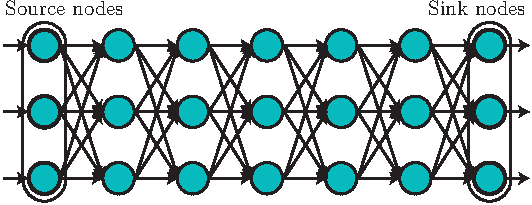
\includegraphics{figures/multiflow.pdf}
	\caption{A ``layered'' flow graph. The graph only shows the edges for one commodity.}
	\label{fig:multiflow}
\end{figure}

It consists of seven layers with three nodes each, and there are two commodities. From each node at a given level, there is a directed edge to each node at the next level. Sources are composed of the nodes at the first level, while the nodes at the last level constitutes the sinks. The capacity for each commodity $c_i$ and edge $e$ is 0 with a probability of 5\% and otherwise drawn from a uniform distribution between 5 and 15, while the common capacity of the edge e is 0 with probability 25\% and otherwise a number drawn from the uniform distribution between $s$-10 and $s$, where $s$ is the sum of the individual capacities on that edge. Similarly to Table~\ref{tab:projections}, Table~\ref{tab:multicom} shows the size of the original model (both as modelled and presolved) and the projections resulting from a flat and decomposed projection, respectively. Both projections finished and the time taken to make them is also shown. Figure~\ref{fig:multicom} shows the progression over time of the number of inequalities and number of variables left to be projected, for both the flat and decomposed projection algorithm.

\begin{table}[htbp]
\centering
\begin{tabular}{l|r@{ / }r@{ / }r@{ / }r|r}
\toprule
$\multirow{2}{*}{Model}$&\multicolumn{4}{c|}{Size}&{Time}\\
&ineqs (eqs)&vars&non-zeros&density&\\
\midrule
Original&204 (42)& 120& 444&2.17&-\\
Presolved& 59& 79& 201&3.41&-\\
Projected, decomposed& 17 (2)& 12& 61&3.59& 2h \phantom{9}9m \\
Projected, flat& 17 (2)& 12& 53&3.12& 17h 41m\\
\bottomrule
\end{tabular}
\caption{Size of projection of a multi-commodity flow model.}
\label{tab:multicom}
\end{table}

Also here we see a reduction in the number of inequalities, variables and non-zero entries, of 3.5, 6.6, and 3.3/3.8 times, respectively (in both cases) compared to the presolved model. The density stays almost the same; for the decomposed model, the density increases with 5.3 \%, while the density decreases with 8.5\% for the flat projection.
This is not as big a reduction as for the VSMs, however, the unprojected models are also smaller to begin with. 
\begin{figure}
	\centering
		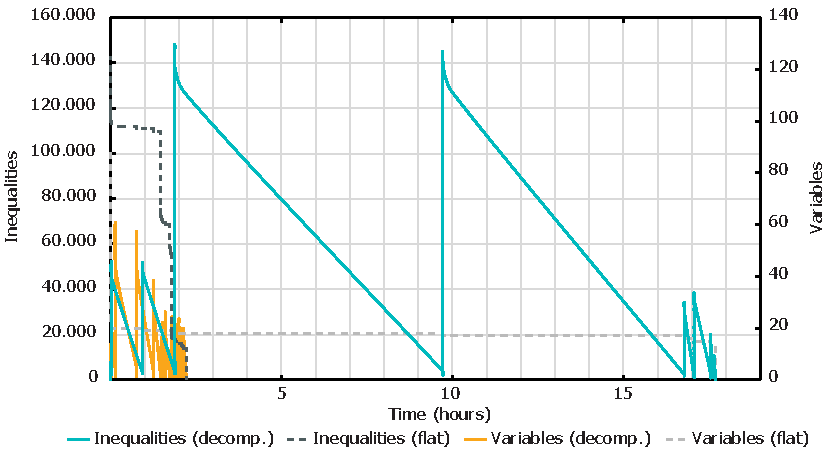
\includegraphics[scale=0.7]{figures/multicomGraph2.pdf}
	\caption{The number of constraints and variables as a function of time during a flat and and a decomposed projection, respectievly, of a multi-commodity flow problem.}
	\label{fig:multicom}
\end{figure}

%%%%%%%%%%%%%%%%%%%%%%%%%%%%%%%%%%%%%%%%%%%%%%%%%%%%%%%%%%%%%%%%%%%%%%%%%%%%%%%%%%%%%%%%%%%%%%%%%%%

\section{Related Work}
\label{sec:preWork}
Previous work on stowage planning optimization (e.g., \cite{roach00,kimkang02,ambrosino04,low09,delgado09,pacino12}) has contributed frameworks for automated stowage planning, and recently, linear stowage planning models were shown to scale to large container vessels (\cite{pacino11,AlbertosThesis}). Since these models define the set of legal stowage conditions, they can be used to compute the residual capacity of a container vessel as a result of the interaction between the different types of containers to load. In other words, they embed an accurate capacity model. 

However, the use of these stowage models as capacity models is limited due to their size. Since a stowage model not only models the capacity of a vessel as a function of the different container types to load but also describes the position of the containers on the vessel, it may contain tens of thousands of constraints and variables and take long time to solve. This is a problem if the stowage model is to be used as a capacity model in uptake-, capacity-, fleet-, and network management, since these tasks often require several hundred capacity models to be solved simultaneously. For example, the task in uptake management of maximizing uptake over a set of voyages, requires us to associate a capacity model with each individual leg of the voyages and then optimize the resulting model.  

Our FME-based framework for variable elimination is to our knowledge the first that can take advantage of block-angular structure in the system. In \cite{simon05} Simon and King combine FME, Gauss-elimination, removal of linearly dependent inequalities and complete redundancy removal in a similar fashion as we have done, to project sparse systems. Moreover, they use the extreme point method of Huynh \textit{et al.} \cite{huynh92} to make approximations of the projection when this is necessary. Their method is implemented as part of an argument-size analyzer for logic programs and tested on a variety of these. Their elimination procedure is therefore not applied once, but instead multiple times during an analysis, and their method and results are for that reason hard to compare to ours. The (in)equality systems operated on are rather sparse and quite small, while their objective is to do the analysis more efficiently (faster) than other methods (when using the polyhedral abstract domain for program analysis). 

Lukatskii and Shapot \cite{lukatskii08}, \cite{shapot12} describe and implement a projection method using FME augmented with \v{C}ernikov's rules. They further use techniques for full redundancy removal examining the solution matrix for a basic solution. Further, they present and apply a method for ``additional matrix clean up'', where some almost redundant inequalities are removed. Their method for this is a little more elaborate than ours and involves a successive increase of the allowable deviation (corresponding to our $\epsilon$) and a permissible maximal ratio between the number of inequalities in the current system compared to the original system. They perform tests on a prototype implementation, where the size ranges between $81$ inequalities and $40$ variables to $201$ inequalities and $100$ variables, i.e., the systems they project are much smaller than the ones we have considered; granted, their run time is also smaller than ours. 

Separately, particularly within linear programming, work has also been done in the area of classifying and removing redundant inequalities in a inequality system as well as finding implicit equalities, e.g. \cite{telgen83}, \cite{lassez93}, \cite{karwan83}, \cite{andersen95}, \cite{mattheiss73} to name a few. 
Many of these (e.g. \cite{telgen83} and the {majority} of the methods presented in \cite{karwan83}) are to be performed within the simplex procedure (used to optimize an LP) or use the objective function and/or the optimal extreme point for the LP, and are hence not applicable for us. On the other hand, we have used cheap redundancy-identifications e.g. described in \cite{andersen95}, \cite{brearley75} and \cite{maros} in our preprocessing and clean-up method, as well as the removal of linearly dependent inequalities from \cite{lassez93}.

Other methods exist for computing the projection of a feasible area of an (in)equality system, that are not based on FME. For example, in \cite{huynh92}, the authors describe a method (based on a method from \cite{lassez90}) that they recommend for dense systems, called the extreme point method. The method works by finding the extreme points of the polytope $P$ defined by the convex combinations of constraints in $S$ that eliminate the variables in $Y$. Since the method finds extreme points and hence inequalities in the projection space incrementally, the method can be used to approximate the projection. The method is consequently used as a supplement to FME, Gauss elimination and full redundancy removal in \cite{simon05}, when the system being projected becomes too dense and an approximation is required.

Huynh, Lassez and Lassez \cite{huynh92} further describe a method (based on \cite{lassezlassez}), the convex hull method, in which the projection of an inequality system $S$ is computed by successive refinements of an initial approximation of the projection. According to the authors, the complexity of their algorithm ``depends essentially on the dimension of the projection of the output not the size of the input'' \cite{huynh92}, and could therefore be an interesting alternative to Fourier-Motzkin-elimination in a case like the one we consider. Another example is the method introduced in \cite{jones04}, called equality set projection, which computes all facets of the projection by first finding a random facet and then iteratively computing all adjacent facets (without revisiting them) {using a face-lattice}. 
This method is recommended by the authors for polytopes with a low facet count and a high vertex count.

\section{Conclusion}\label{sec:concl}
For a liner shipping company, accurate capacity models that succinctly represent the trade-off between the different types of containers are important in many areas such as uptake management, capacity management, network management, and fleet management. Although previous work on stowage models in principle provide fine-grained capacity models, they cannot readily be used in practice as such, since they are too large.
As an alternative, we have developed a framework based on Fourier-Motzkin elimination that automatically translates a linear stowage model (VSM) into a smaller sized capacity model (VCM) by projecting unneeded variables. The framework utilizes preprocessing, variable elimination (FME and Gauss-elimination), a parallel redundancy removal, as well as a boundary coarsening (removal of almost redundant inequalities). It uses a novel decompostion method that exploits the block-angular structure of the problem to speed up the projection.

Our results show that the projected VCMs are reduced by an order of magnitude both in number of inequalities and number of non-zero entries. The VCMs including hydrostatic constraints are solved 20-35 times faster than their corresponding VSMs, while the difference in objective value is 0.15-0.5 \%. For the models not including hydrostatic constraints, the speed-up is larger, but so is the loss of accuracy. The more realistic models including hydrostatic constraints are therefore more suited as submodels in optimization tasks within e.g. capacity management. 

Our framework makes use of a decomposition of the block-angular structure of the VSMs, and this decomposition drastically improves the runtime of the projections of the more complex stowage models. The block-angular structure is commonly found in real-world linear models, and our projection framework can be used for other problems. As an example, we have considered a multi-commodity flow problem and applied our framework. We found a similar speed-up as for the VSMs. 

There are several interesting directions for future work. 
From an application point of view, it could be interesting to test the VCMs in an actual setting for e.g. uptake management in a flow graph.
Likewise it could be interesting to  add more constraints to the VSM and/or investigate the limits for the decomposition framework. Of course, in this connection, various optimizations of the framework and its implementation, such as e.g. the mentioned parallellization of the projection of the subsystems of the decomposed system, would be useful to enhance the framework and further speed up the projection. Finally, for using the decomposition for different problems, it would be useful to have a procedure, that automatically estimates the best way of decomposing a given system. Finding and testing the framework on more block-angular problems in need of projection would also be of interest.

\subsection*{Acknowledgements}
We would like to thank Stefan R{\o}pke, Thomas Stidsen, and David Pisinger for discussions on applications of the FME framework beyond container vessel capacity models. This research is supported by the Danish Maritime Fund, Grant No. 2016-064.

\bibliography{bibfile}{}
\bibliographystyle{alpha}

\end{document}
